\section{Matrix Factorization}
As discussed above, to reduce the gap between predicted rating $\hat{r}_{u,i}$ and real rating $r_{u,i}$, \textit{root mean square error} (RMSE) is used as the loss function and $\mathit{l}_{2}$ norm is adopt as the regularization term. Then, when we already have the loss function, the next step is to minimize the loss function. Here we use the stochastic gradient descent (SGD) method to minimize the loss function. Next, the derivation of stochastic gradient descent will be provided. By Taylor expansions, we have the following equation:
\begin{equation}
    f(\theta) \approx f\left(\theta_{0}\right)+\left(\theta-\theta_{0}\right) \cdot f^{\prime}\left(\theta_{0}\right)
\end{equation}
where $\left(\theta-\theta_{0}\right)$ is a vector, it represents the distance of change. We can denote it by $\eta $. $\eta $ is a scalar, and the unit vector of $\left(\theta-\theta_{0}\right)$ is expressed by $v$:
\begin{equation}
    \left(\theta-\theta_{0}\right) = \eta \cdot v
\end{equation}
By formula 3.2, the formula 3.1 can change as:
\begin{equation}
        f(\theta) \approx f\left(\theta_{0}\right)+\eta v \cdot f^{\prime}\left(\theta_{0}\right)
\end{equation}
To minimize the loss function, we need minimize the $f(\theta)$. In other words, we want to make the value of the $f(\theta)$ smaller each time we update the $\theta$. So that $f(\theta)-f\left(\theta_{0}\right)< 0$, by this we have:
\begin{equation}
    f(\theta)-f\left(\theta_{0}\right) \approx \eta v \cdot f^{\prime}\left(\theta_{0}\right) < 0
\end{equation}
Where, $\eta $ is scalar and generally positive, which can be ignored. Therefore:
\begin{equation}
    v \cdot f^{\prime}\left(\theta_{0}\right) < 0
\end{equation}
From vector multiplication, when the angle between two vectors is 180 degrees, the product of vector multiplication is less than 0, and minimal. So, when the direction of $v$ and $f^{\prime}\left(\theta_{0}\right)$ is opposite (i.e. included angle is 180 degrees), $v \cdot f^{\prime}\left(\theta_{0}\right) < 0$ and have minimal value. From this we can get: 
\begin{equation}
    v=-\frac{f^{\prime}(\theta)}{\left\|f^{\prime}(\theta)\right\|}
\end{equation}
where $v$ is a unit vector, so we divide it by the norm of the $f^{\prime}(\theta)$, substitute the formula 3.6 into formula 3.2:
\begin{equation}
    \theta=\theta_{0}-\eta \frac{f^{\prime}(\theta)}{\left\|f^{\prime}(\theta)\right\|}
\end{equation}
Due to the norm of a vector being a scalar, we obtain:
\begin{equation}
    \theta=\theta_{0}-\eta f^{\prime}(\theta)
\end{equation}
where $\theta_{0}$ is is the current parameter, $\eta$ denote the stride or so call learn rate, $f^{\prime}(\theta)$ is the direction of the gradient.
However, our loss function is a multivariate function, so we need to calculate the partial derivatives of it. So the formula of $\theta$ become:
\begin{equation}
    \theta=\theta_{0}-\eta  \frac{\partial}{\partial \theta_{0}} J(\theta)
\end{equation}
For our loss function,
\begin{equation}
        \text { Loss }: J(p, q)=\min_{ q *, p * } \sum_{(u, i) \in K}\left(r_{u,i}-q_{i}^{T} p_{u}\right)^{2}+\lambda\left(\left\|q_{i}\right\|+\left\|p_{u}\right\|\right)^{2}
\end{equation}
Where $q_{i}$ and $p_{u}$ are the variables which need to optimize, $\lambda$ is the regularization factor. Our goal is to optimize the $q_{i}$ and $p_{u}$ and find the minimum value of the loss function.
Perform partial derivative on both $q_{i}$ and $p_{u}$:
    \begin{equation}
        \frac{\partial E}{\partial q_{i}}=-2\left(r_{u,i}-q_{i}^{T} p_{u}\right) p_{u}+2 \lambda q_{i}
    \end{equation}
    \begin{equation}
        \frac{\partial E}{\partial p_{u}}=-2\left(r_{u,i}-q_{i}^{T} p_{u}\right) q_{i}+2 \lambda p_{u}
\end{equation}
Substituted two partial derivatives into the gradient descent formula 3.9:
\begin{equation}
    q_{i}=q_{i}+2 \eta\left(\left(r_{u,i}-q_{i}^{T} p_{u}\right) p_{u}-\lambda q_{i}\right)
\end{equation}
\begin{equation}
    p_{u}=p_{u}+2 \eta\left(\left(r_{u,i}-q_{i}^{T} p_{u}\right) q_{i}-\lambda p_{u}\right)
\end{equation}
By define $e_{u,i}=r_{u,i}-q_{i}^{T} p_{u}$. we have:
\begin{equation}
    q_{i} \leftarrow q_{i}+\eta\left(e_{u,i} p_{u}-\lambda q_{i}\right)
\end{equation}
\begin{equation}
    p_{u} \leftarrow p_{u}+\eta\left(e_{u,i} q_{i}-\lambda p_{u}\right)
\end{equation}
To sum up, the above process is the derivation process of stochastic gradient descent.By the stochastic gradient descent algorithm, we train two latent vector matrices: user matrix \textit{p} and item matrix \textit{q}. Through the inner product of user matrix \textit{p} and item matrix \textit{q}, we can have the predicted user-item matrix. If the user matrix and item matrix are fitted by the loss function perfectly, then our predicted rating will be infinitely close to the real rating. 

In this project, we consider another scenario in which some harsh users give a low rating, but some users are more tolerant, giving a relevant high score for bad items. By this intuition, we trying to add bias into matrix factorization.
\begin{equation}
        \hat{r}_{u,i}=\underset{basic}{\underbrace{q_{i}^{T}p_{u}}}+ \underset{bias}{\underbrace{b_{ui}}}
    \end{equation}
So that our predicted rating become:
\begin{equation}
    \hat{\boldsymbol{r}}_{u,i}=b_{u,i}+q_{i}^{T} * p_{u}
\end{equation}
And the loss function is:
\begin{equation}
    \operatorname{Loss}=\min _{q^{*}, p^{*}} \sum_{(u, i) \in K}\left(r_{u,i}-b_{u,i}-q_{i}^{T}p_{u}\right)^{2}+\lambda \left(\left\|q_{i}\right\|^{2}+\left\|p_{u}\right\|^{2}+b_{u}^{2}+b_{i}^{2}\right)
\end{equation}
where $b_{u,i} = \mu+b_{u}+b_{i}$. We use $\mu$ to denote the average rating for the entire rating matrix, $b_{u}$ denote the user's bias, and $b_{i}$ is represent the item bias.
In the next chapter, we will simulate these two approaches with real data and evaluate the performance between the two approaches .
\section{Memory-Based Collaborative Filtering Recommender System}
As was pointed out in the formulation of this report, memory-based collaborative filtering makes recommendations based on the similarity between the users or the items. The detailed steps of the memory-based collaborative filtering can be stated as follows:
\begin{itemize}
    \item[1. ]Identify a target user who will be recommended.
    \item[2. ]Figure out the items that the target user has given ratings for.
    \item[3. ]Based on the target user’s rating pattern, find similar users.
    \item[4. ]Get the rating records of similar users for items.
    \item[5. ]Calculate the similarity between the target user and a similar user by formula (e.g., \textit {Euclidean Distance}, \textit{Pearson Correlation}, \textit{Cosine Similarity}).
    \item[6. ]Recommend the items with the highest score to the target user.

\end{itemize}
In the following, an example will be demonstrated to elaborate on the above steps.
\begin{figure}[htbp]
\centering
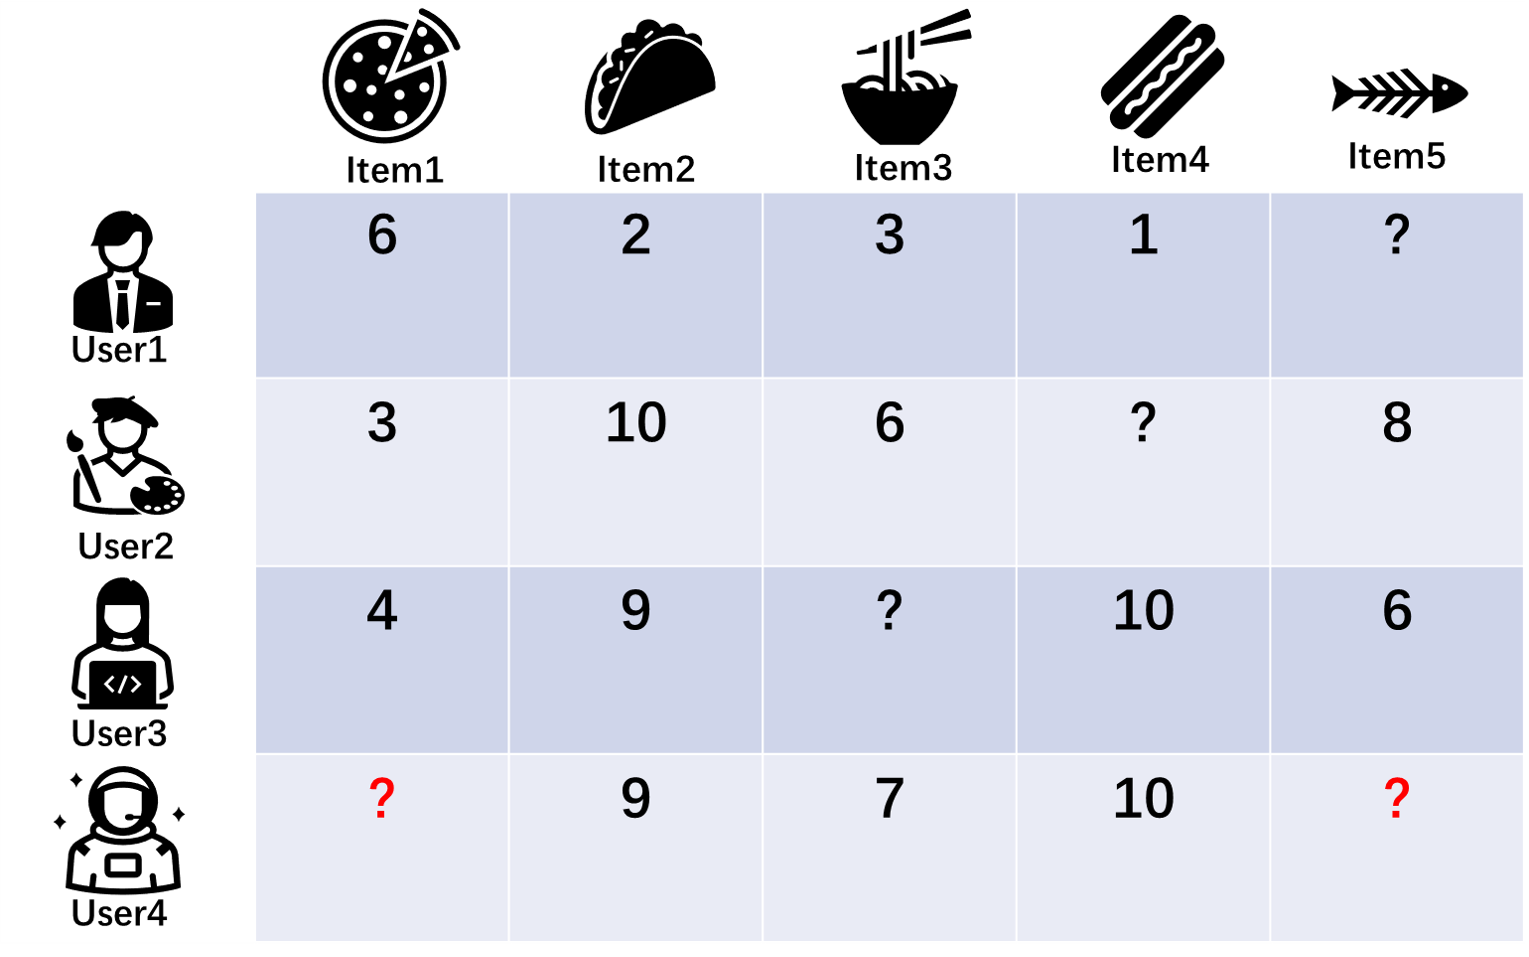
\includegraphics[scale=0.55]{figure/rating1.png}
\caption{Example of User$-$item rating matrix}
\end{figure}

As per the user-item rating matrix shown in Figure 3.1, assume \textit{user4} is our target user and rated three out of five items. The goal of the system is to figure out which one of the two unrated items (i.e., \textit{item1} and \textit{item5}) should be recommended to the target user who can probably get a high rating. After we define our target user and figure out some users, the next step that comes up is to calculate the similarity between the target user and similar users. The common methods of similarity calculation include \textit{Euclidean Distance}, \textit{Pearson Correlation}, \textit{Cosine Similarity}. To calculate the similarity between two users, we base it on the ratings of \textit{item2}, \textit{item3}, and \textit{item4} which are the items that all users have rated.
\begin{figure}[htbp]
\centering
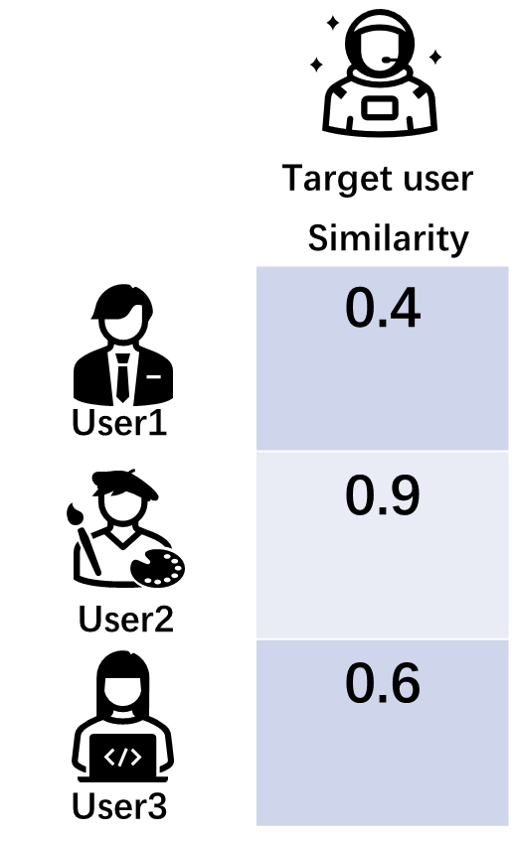
\includegraphics[scale=0.5]{figure/rating2.png}
\caption{Similarity between target user and other users}
\end{figure}
Here we make a hypothesis that the similarity between the target user and other users is 0.4, 0.9, and 0.6, respectively, as shown in Figure 3.2. The next step is that, based on the value of similarity, we can calculate the predicted rating for the target user. What can be seen in Figure 3.3 is the so-called weighted rating matrix because it provides more weight to those users who have a higher similarity to the target user.
\begin{figure}[htbp]
\centering
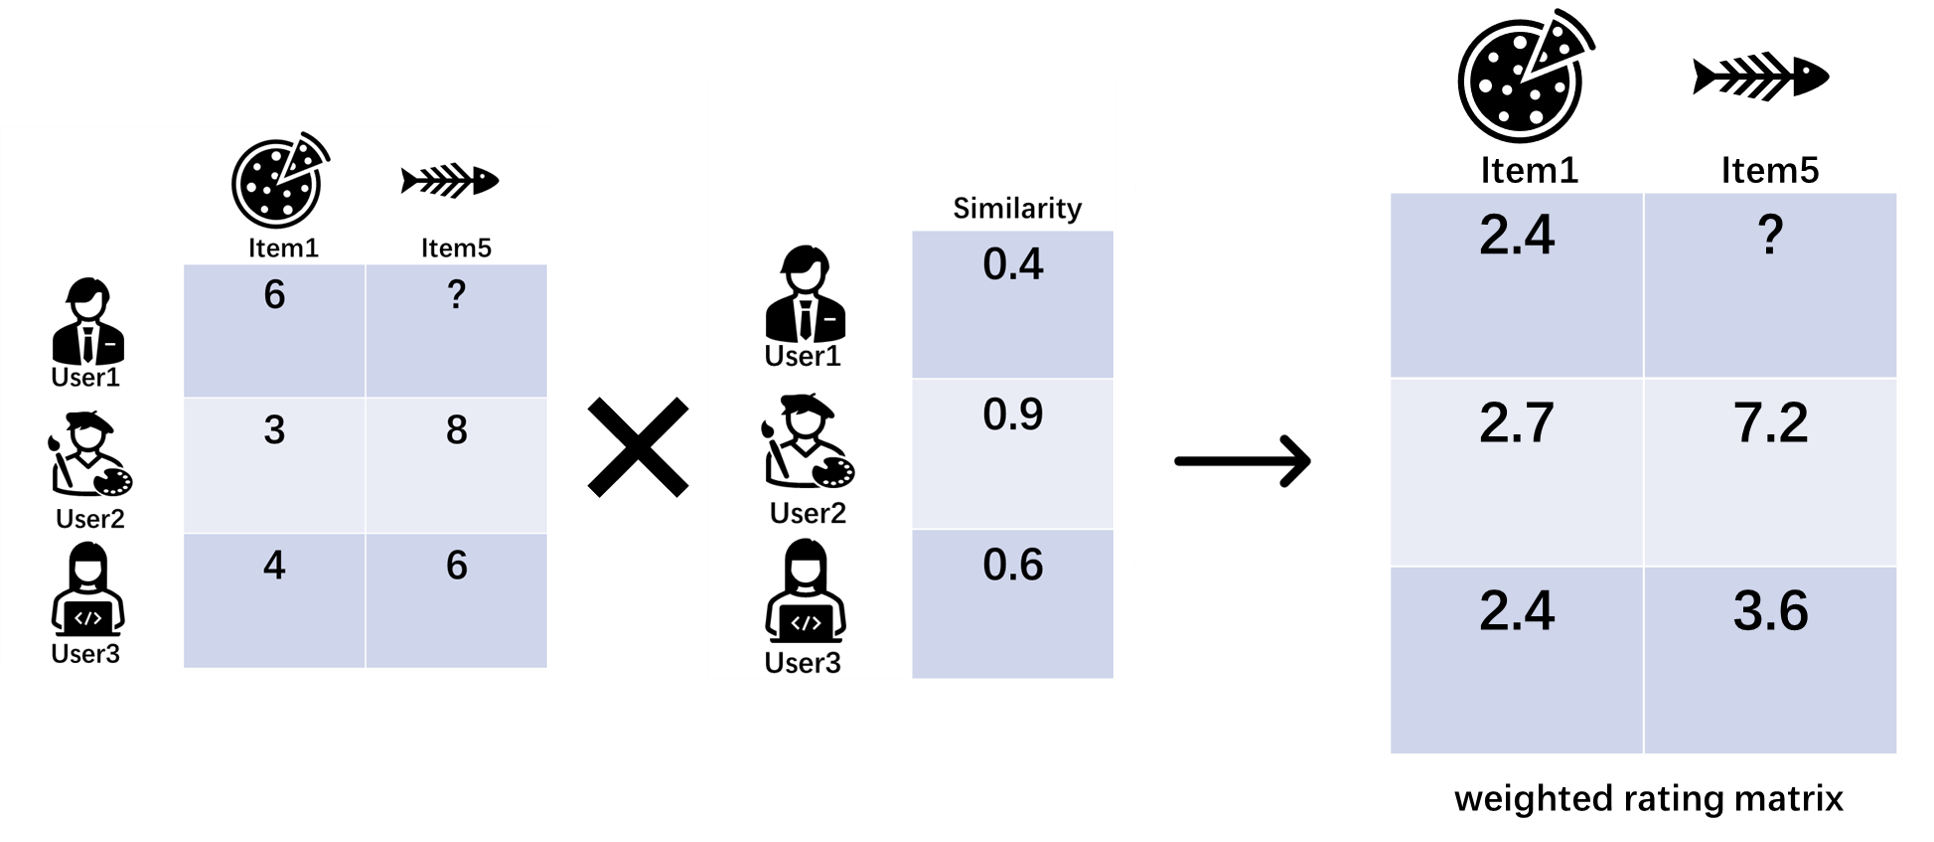
\includegraphics[scale=0.5]{figure/rating3.png}
\caption{Weighted rating matrix}
\end{figure}
For the final step, we tally up all weighted rates to create the recommender matrix. Due to the sparsity of the weighted rating matrix (e.g. only \textit{user2} and \textit{user3} provided the rating for \textit{item5} , we normalize the value of the weighted rating by dividing the sum of weighted ratings by the sum of the similarity for users.
\begin{figure}[htbp]
\centering
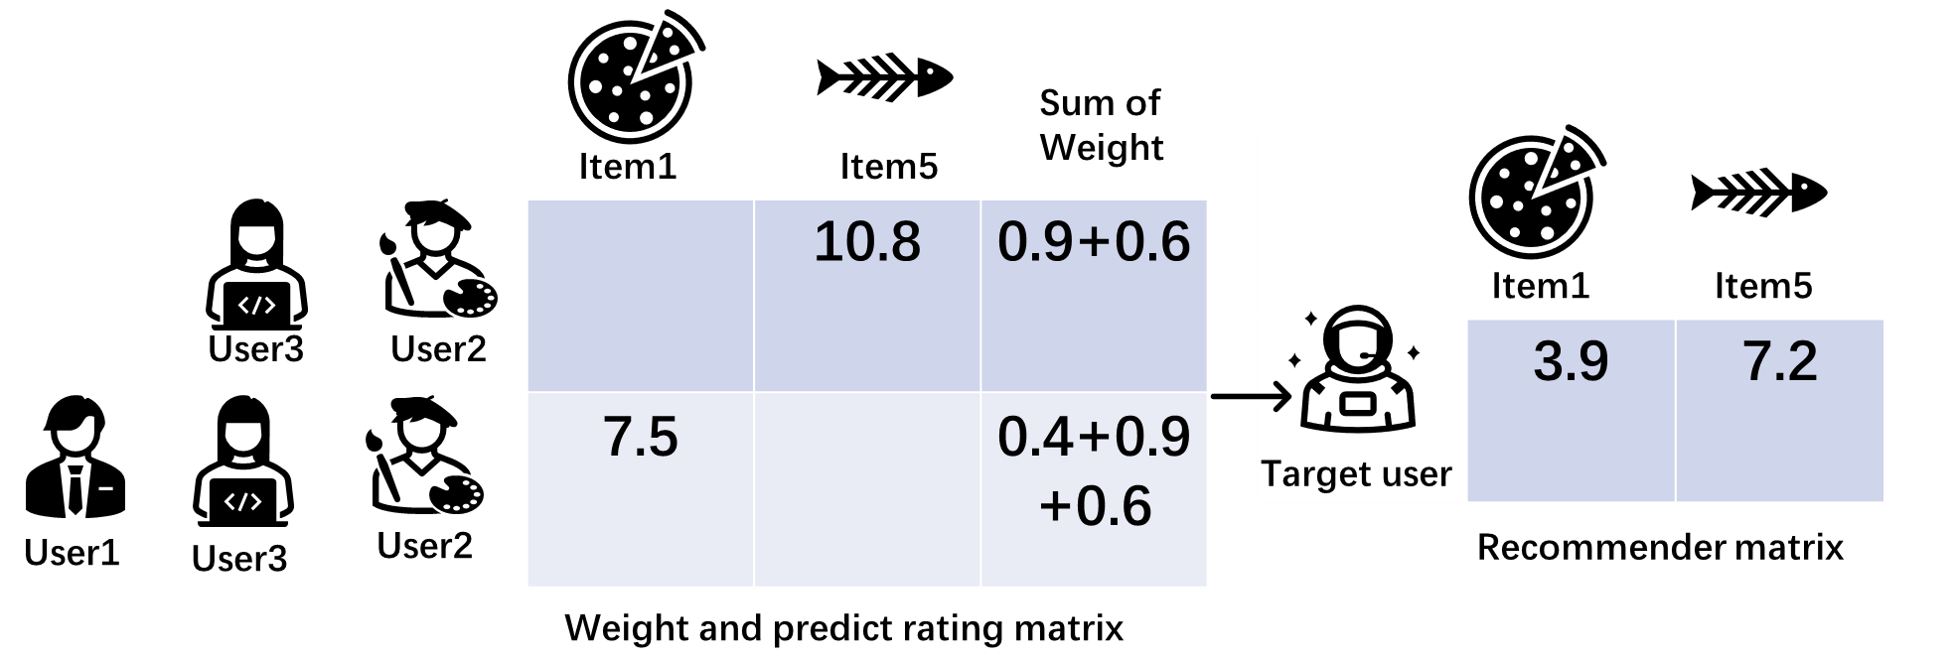
\includegraphics[scale=0.5]{figure/rating4.png}
\caption{Recommender matrix}
\end{figure}
According to the result of user-based collaborative filtering shown in Figure 3.4, the value in the recommender matrix describes the potential rating for the target user that will arise for the items based on the similarity between them and other users. The target user potentially provides a higher rating to \textit{item5} than \textit{item1}. So, through the result, the user-based collaborative filtering recommender system will choose \textit{item5} to recommend to the target user.


